
\pdfminorversion=4
\documentclass[xcolor=dvipsnames]{beamer}
\usepackage{tabls}
\usepackage{graphicx}
\usepackage{xcolor}
\usepackage{mathtools}
%\usepackage{subcaption}

%tikz stuff
\usepackage{tikz}
\usetikzlibrary{shapes.geometric, arrows}
\tikzstyle{startstop} = [rectangle, rounded corners, minimum width=2cm, text
    width=1.8cm, minimum height=1cm,text centered, text=white,draw=black, fill=Gray!140]
\tikzstyle{io} = [trapezium, trapezium left angle=70, trapezium right angle=110,
minimum width=0.5cm, minimum height=1cm, text centered, draw=black,
fill=blue!20!Gray!90!,text=white]
\tikzstyle{process} = [rectangle, minimum width=2cm, minimum height=1cm, text
centered, text width=2cm, draw=black, text=white,fill=Gray!140!blue!70!white]
\tikzstyle{decision} = [diamond, minimum width=3cm, minimum height=1cm, text
centered, draw=black, fill=Gray!,text=white]
\tikzstyle{arrow} = [thick,line width=0.6mm,->,>=stealth]
\tikzstyle{arrow1} = [dashed,->,>=stealth]

\setbeamertemplate{navigation symbols}{}
\setbeamertemplate{footline}[frame number]
%\setbeamertemplate{headline}{}
\setbeamersize{text margin left=15pt,text margin right=15pt}

\definecolor{mylightlue}{rgb}{1,1,1}
\newcommand*{\boxedcolor}{red}
\makeatletter
\renewcommand{\boxed}[1]{\textcolor{\boxedcolor}{%
  \fbox{\normalcolor\m@th$\displaystyle#1$}}}
\makeatother
\usepackage{hyperref}

\renewcommand{\u}[1]{\underline{#1}}

\newcommand{\iso}[2]{${}^{{#2}}${#1} }
\newcommand{\nubar}[0]{$\overline{\nu}$ }
\newcommand{\keff}[0]{\ensuremath{{k}_{\textsf{eff}}} }
\newcommand{\expect}[1]{E[#1] }
\newcommand{\colg}[1]{{\color{ForestGreen} #1}}
\newcommand{\coly}[1]{{\color{yellow} #1}}
\newcommand{\colb}[1]{{\color{blue} #1}}
\newcommand{\colr}[1]{{\color{red} #1}}
\usepackage{amsfonts}
\newlength{\wideitemsep}
\setlength{\wideitemsep}{8pt}
%\addtolength{\wideitemsep}{5pt}
\let\olditem\item
\renewcommand{\item}{\setlength{\itemsep}{\wideitemsep}\olditem}

\newcommand{\N}{\mathbb{N}}
\newcommand{\Z}{\mathbb{Z}}
\newcommand{\deriv}[2]{\frac{\mathrm{d} #1}{\mathrm{d} #2}}
\newcommand{\pderiv}[2]{\frac{\partial #1}{\partial #2}}
\newcommand{\bx}{\mathbf{X}}
\newcommand{\ba}{\mathbf{A}}
\newcommand{\by}{\mathbf{Y}}
\newcommand{\bj}{\mathbf{J}}
\newcommand{\bs}{\mathbf{s}}
\newcommand{\B}[1]{\ensuremath{\mathbf{#1}}}
\newcommand{\Dt}{\Delta t}
\renewcommand{\d}{\mathsf{d}}
\newcommand{\mom}[1]{\langle #1 \rangle}
\newcommand{\xl}{{x_{i-1/2}}}
\newcommand{\xr}{{x_{i+1/2}}}
\newcommand{\il}{{i-1/2}}
\newcommand{\ir}{{i+1/2}}

\AtBeginSection[]
{
    \begin{frame}<beamer>
        \frametitle{Outline}
        \tableofcontents[currentsection]
    \end{frame}
}

\setbeamerfont{frametitle}{size=\large}
\setbeamerfont{normal font}{size=\small}

\graphicspath{{figures/}}

\usepackage{verbatim}
\usepackage{comment}
\usepackage[]{datetime}
\usepackage{multirow}

\usepackage[]{color}
\usepackage{geometry}

\mode<presentation>
\usepackage{multimedia}

\usepackage{xcolor}


\newcommand{\thedate}{\today}


\setlength{\tabcolsep}{.25cm}

%Aggie-themed
%\pgfdeclareimage[height=0.1in]{TAMUlogo}{tamu_engineering.png}
%\logo{\raisebox{-0pt}{\pgfuseimage{TAMUlogo}}}
%\titlegraphic{\centering\begin{tabular}{lr}\includegraphics[height=0.32\textheight]{../graphic/TAMUlogo.png}\end{tabular}}


%%%%%%%%%%%%%%%%%%%%%%%%%%%%%%%%%%%%%%%%%%%%%%%%%%%%%%%%%%%%%%%
% Optional packages, used to show off certain tricks

\newlength \figwidth
\setlength \figwidth {0.5\textwidth}

\setlength{\leftmargin}{0cm}
\setlength{\rightmargin}{0cm}

%%%%%%%%%%%%%%%%%%%%%%%%%%%%%%%%%%%%%%%%%%%%%%%%%%%%%%%%%%%%%%%

\usepackage[english]{babel}
\usetheme{Frankfurt}

%Make it Aggie Maroon
\usecolortheme[RGB={80,0,0}]{structure}  

  % This will typeset only the frames (or slides) that have the given label ("current" in this case).

\title{The Coarse Scattering Method}
%\author{Pablo A. Vaquer}

\begin{document}

%\begin{frame}
%    \titlepage 
%    \begin{center}
%\begin{figure}[ht]
%\begin{subfigure}
%
\includegraphics[width=.33\textwidth]{./graphics/ans-logo.png}
%\end{subfigure}
%\begin{subfigure}
%  \centering
%
\includegraphics[width=.33\textwidth]{./graphics/tamu.jpg}
%\end{subfigure}
%\end{figure}
%    \end{center}    
%\end{frame}

\begin{frame}
\frametitle{Purpose}

\begin{itemize}
\item The purpose is to reduce the computational time for multigroup (MG) transport simulations
\item The scatter and fission transfer matrices are mapped onto a coarse energy grid, the sourced-particle flux is then mapped back onto the fine MG energy grid
\end{itemize}

\end{frame}


\begin{frame}
  \frametitle{Introduction: neutron transport equation}

The neutron transport equation is
\begin{multline*}
\label{eq:transport}
\frac{1}{v(E)} \frac{\partial \psi}{\partial t} + \hat{\Omega} \cdot \nabla \psi+ \Sigma_{t}(\vec{r},E,t) \psi(\vec{r},\hat{\Omega},E,t) = \\q(\vec{r},\hat{\Omega},E,t) + \sum_{i=1}^I \frac{\chi_{d,i}(E)}{4 \pi} \lambda_i C_i(t) +  \frac{1}{4 \pi} \int_0^\infty dE' \,  \Sigma_{pf}(\vec{r},E' \to E) \phi(\vec{r},E',t) \, + \\ \sum_{\ell=0}^L \sum_{m=-\ell}^\ell \frac{2 \ell + 1}{4 \pi} Y_\ell^m(\hat{\Omega}) \int_0^\infty dE' \,  \Sigma_{s,\ell}(\vec{r},E' \to E) \phi_{\ell}^m(\vec{r},E',t) .
\end{multline*}

\pause

\vspace{0.5cm}

The multigroup (MG) method discretizes energy into groups
\begin{equation*}
\label{eq:transport}
\Sigma_g \phi_g = \int_{E_{g}}^{E_{g-1}} dE \,\Sigma(E) \phi(E) .
\end{equation*}

\end{frame}

\begin{frame}
  \frametitle{Background: the multigroup method}

MG tries to also preserve the scattering reaction rates, as well as the energy and angular distribution of scattered neutrons
\begin{multline*}
 \sum_{\ell=0}^\infty \sum_{m=-\i}^\ell \frac{2 \ell + 1}{4 \pi} Y_\ell^m(\hat{\Omega}) \sum_{g'}^G \Sigma_{s,\ell, g' \to g} \phi_{\ell,g'}^m = \\ \int_0^\infty dE' \,\Sigma_s(\hat{\Omega}' \cdot \hat{\Omega},E' \to E) \psi(\hat{\Omega}',E')
\end{multline*}

Note:
\begin{itemize}
\item Energy is only 1 of the 7 dimensions in neutron transport, so energy is typically discretized into a few hundred groups
\item Computing the scattering source requires $O(G^2)$ operations
\end{itemize}


\end{frame}


\begin{frame}
\frametitle{The coarse scattering method}

In the coarse scattering (CS) method, we make the following substitution to the MG transport equation to reduce the size of the scattering matrices
\begin{equation*}
\label{eq:scatter}
\sum_{g'} \Sigma_{s,\ell,g'\to g} \phi_{\ell,g'} \quad \to \quad S_{\ell,e\to g} \sum_{e'} \Sigma_{s,\ell,e'\to e} \phi_{\ell,e'} 
\end{equation*}
where each fine-group $g$ is a subset of a coarse-element $e$ and
\begin{equation*}
\label{Eq.S}
S_{\ell,e\to g}  = \frac{\sum_{g'} \Sigma_{s,\ell,g'\to g} \phi_{\ell,g'}}{ \sum_{e'} \Sigma_{s,\ell,e'\to e} \phi_{\ell,e'}} 
\end{equation*}
%\begin{equation*}
%\Sigma_{s,\ell,e'\to e} = \sum_{g \in e} \sum_{g' \in e'} \Sigma_{s,\ell,g'\to g} 
%\end{equation*}
\begin{equation*}
\phi_{\ell,e} = \sum_{g \in e} \phi_{\ell,g} 
\end{equation*}

\end{frame}

\begin{frame}
\frametitle{The CS method can also be applied to the fission matrix}


For fission, we make the following substitution
\begin{equation*}
\label{eq:fission}
\sum_{g'} \Sigma_{f,g'\to g} \phi_{g'} \quad \to \quad  F_{e\to g} \sum_{e'} \Sigma_{f,e'\to e} \phi_{e'} 
\end{equation*}
where 
\begin{equation*}
\label{Eq.S}
F_{e\to g}  = \frac{\sum_{g'} \Sigma_{f,g'\to g} \phi_{g'}}{ \sum_{e'} \Sigma_{f,e'\to e} \phi_{e'}} 
\end{equation*}
%\begin{equation*}
%\Sigma_{f,e'\to e} = \sum_{g \in e} \sum_{g' \in e'} \Sigma_{f,g'\to g}
%\end{equation*}
\begin{equation*}
\phi_{e} = \sum_{g \in e} \phi_{g} 
\end{equation*}

\end{frame}


\begin{frame}
  \frametitle{Example of fine transfer matrix being decomposed into a coarse transfer matrix and mapping operator}

\begin{figure}[ht]
  \centering
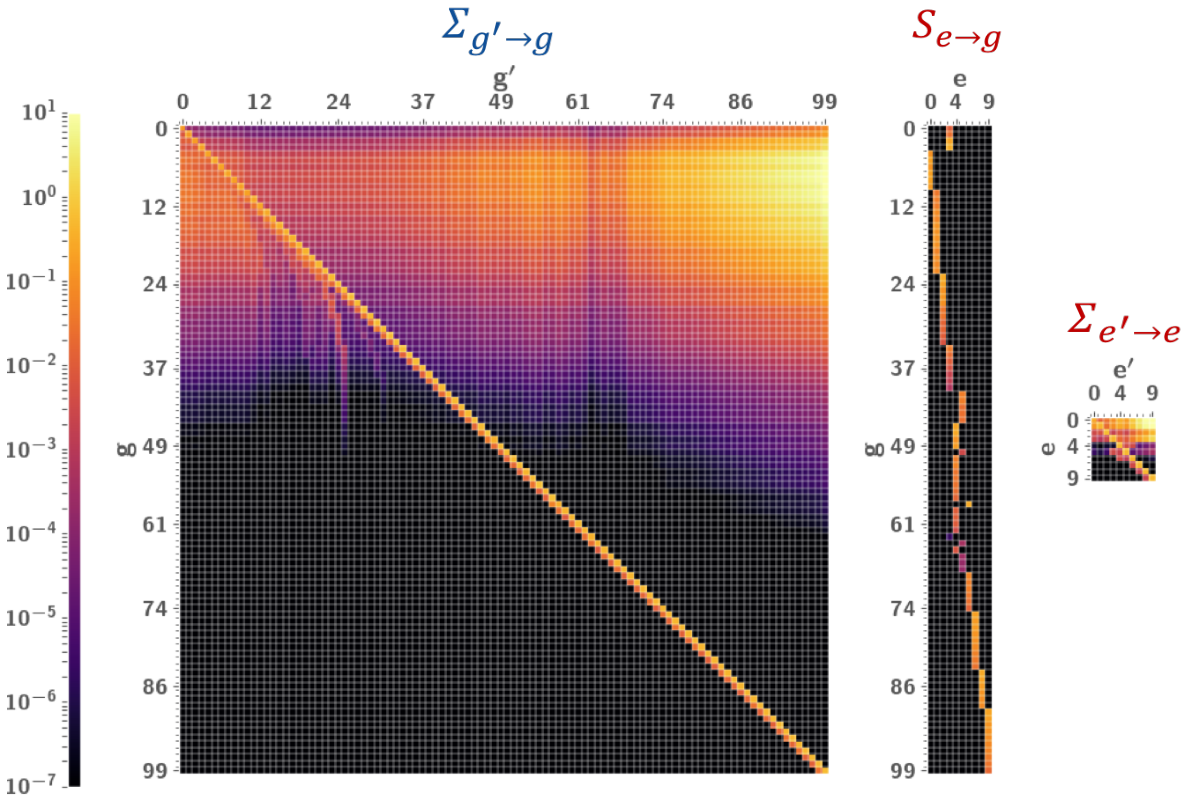
\includegraphics[width=.9\textwidth]{./graphics/matrix_decomposition.png}
\end{figure}
\end{frame}

\begin{frame}
  \frametitle{The standard source iteration method for MG}

\begin{itemize}
\end{itemize}
\begin{multline*}
\Bigg[\frac{1}{v_g} \frac{\partial}{\partial t} + \mu \frac{\partial}{\partial x} + \Sigma_{t,g}(\vec{r},t) \Bigg] \psi^{(i+1)}_g(\vec{r},\mu,t)  = q_g(\vec{r},\hat{\Omega},t) + \\  \sum_{\ell=0}^L \frac{2 \ell + 1}{2} P_\ell(\mu) \sum_{g'}^G \Sigma_{s,\ell, g' \to g}(\vec{r},t) \phi^{(i)}_{\ell,g'}(\vec{r},t) + \\  \frac{1}{2} \sum_{g'}^G \Sigma_{f,g' \to g}(\vec{r},t) \phi^{(i)}_{g'}(\vec{r},t)
\end{multline*}

\vspace{0.5cm}

Recall, the asymptotic computational cost of solving the MG transport equation is order $G^2$

\end{frame}



\begin{frame}
  \frametitle{The source iteration method is modified for CS}

\begin{multline*}
\Bigg[\frac{1}{v_g} \frac{\partial}{\partial t} + \mu \frac{\partial}{\partial x} + \Sigma_{t,g}(\vec{r},t) \Bigg] \psi^{(i+1)}_g(\vec{r},\mu,t)  = q_g(\vec{r},\hat{\Omega},t) + \\  \sum_{\ell=0}^L \frac{2 \ell + 1}{2} P_\ell(\mu) S_{\ell,e\to g}^{(i-s)} \sum_{e'}^E \Sigma_{s,\ell, e' \to e}(\vec{r},t) \phi^{(i)}_{\ell,e'}(\vec{r},t) + \\  \frac{F_{e \to g}^{(i-f)}}{2} \sum_{e'}^E \Sigma_{f,e' \to e}(\vec{r},t) \phi^{(i)}_{e'}(\vec{r},t)
\end{multline*}

Note:
\begin{itemize}
\item It's not necessary to recompute both $S_{\ell,e\to g}$ and $F_{e \to g}$ every iteration
\item Asymptotic computational cost of the CS method is order $G$ in iterations when $S_{\ell,e\to g}$ and $F_{e \to g}$ are not recomputed and order $G^2$ only in iterations where $S_{\ell,e\to g}$ and $F_{e \to g}$ are recomputed
\end{itemize}

\end{frame}



\begin{frame}
\frametitle{Particle balance is maintained}
Particle balance is maintained if the following residual $\rho$ is less than some specified tolerance in the last iteration 
\begin{multline*}
\label{eq:scatter}
\rho = \sum_{g}^G \sum_{i}^I \Big[ \Big( \sum_{g'}^G \Sigma_{s,0,g'\to g,i} \phi_{g',i} + \sum_{g'}^G \Sigma_{f,g' \to g,i} \phi_{g',i} \Big) - \\  \Big( S_{0,e\to g,i} \sum_{e'}^E \Sigma_{s,0,e'\to e,i} \phi_{e',i} + F_{e\to g,i} \sum_{e'}^E  \Sigma_{f,e' \to e,i} \phi_{e',i} \Big) \Big]
\end{multline*}

\vspace{0.5cm}

Alternatively, the MG method can be used in the last iteration

\end{frame}

\begin{frame}
  \frametitle{Test problem 1: description}
Determine $k$-eigenvalue for an 8cm thick slab of uranium (20$\%$ enriched)

\vspace{0.5cm}

A $S_N$ code was written in Python to simulate neutron transport and compare MG to CS:
\begin{itemize}
\item 200 energy groups for MG 
\item 200 fine groups / 25 coarse-groups for CS  
\item 20 spatial cells (diamond-difference discretization)
\item 8 polar angles
\item isotropic scattering
\end{itemize}
\end{frame}

\begin{frame}
  \frametitle{Test problem 1: how often the fission and scattering spectra were recomputed}
\begin{itemize}
\item $F_{e \to g}$ recomputed every 8 iterations
\item $S_{0,e \to g}$ recomputed every 2 iterations
\end{itemize}
\end{frame}

\begin{frame}
  \frametitle{Test problem 1: results for flux and $k$-eigenvalue}
\begin{itemize}
\item Both MG and CS simulations resulted in a $k = 1.18173$ 
\item The MG simulation converged in 45 iterations and the CS simulation converged in 49 iterations
\item The MG simulation took 60s and the CS simulation took 31s
\end{itemize}

\begin{figure}[ht]
\begin{subfigure}
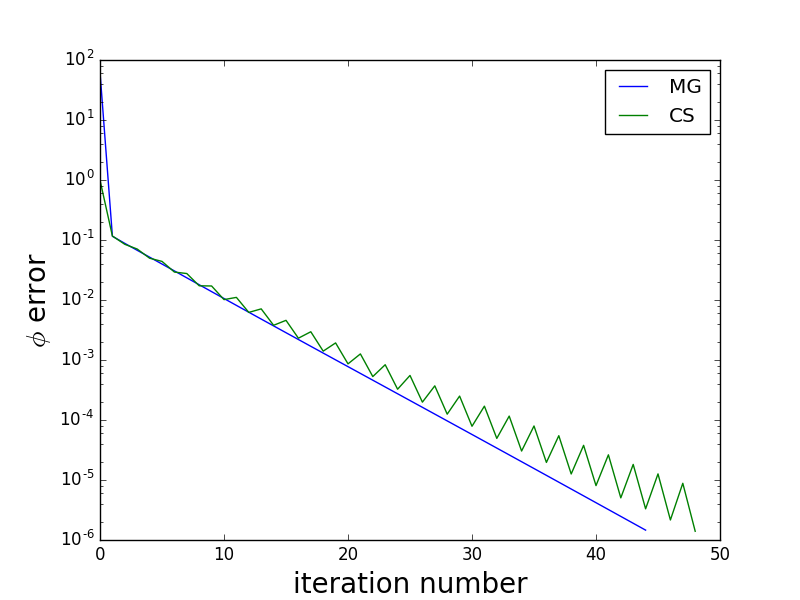
\includegraphics[width=.49\textwidth]{./graphics/phi_error_1.png}
  %\caption{640 MG groups}
\end{subfigure}
\hfill
\begin{subfigure}
  \centering
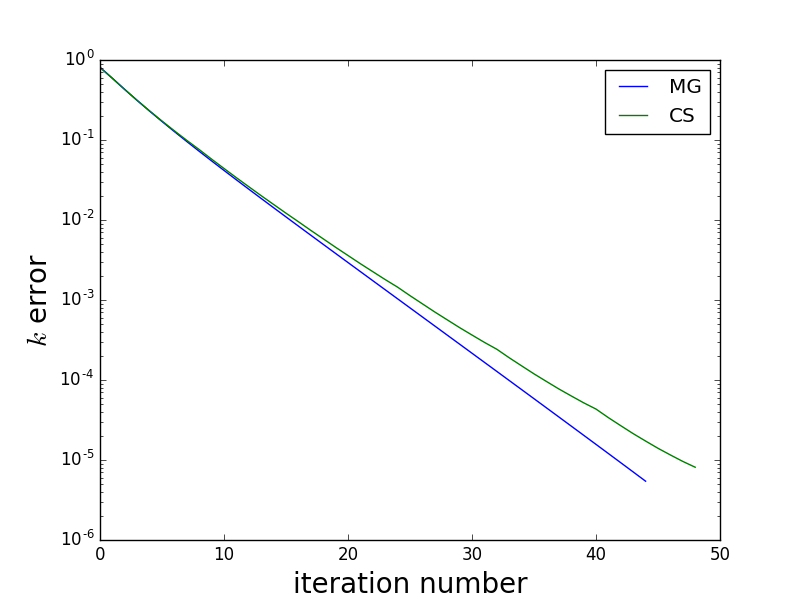
\includegraphics[width=.49\textwidth]{./graphics/k_error_1.png}
  %\caption{640 MG groups}
\end{subfigure}
\end{figure}
\end{frame}

\begin{frame}
  \frametitle{Test problem 2: description}
Determine $k$-eigenvalue for an 8cm thick slab of uranium (20$\%$ enriched)

\vspace{0.5cm}

A $S_N$ code was written in Python to simulate neutron transport and compare MG to CS:
\begin{itemize}
\item 200 energy groups for MG 
\item 200 fine groups / 25 coarse-groups for CS  
\item 20 spatial cells (diamond-difference discretization)
\item \textcolor{blue}{32 polar angles}
\item \textcolor{blue}{$P_7$ scattering}
\end{itemize}
\end{frame}

\begin{frame}
  \frametitle{Test problem 2: how often the fission and scattering spectra were recomputed}
\begin{itemize}
\item $F_{e \to g}$ recomputed every 8 iterations
\item $S_{0,e \to g}$ recomputed every 2 iterations
\item \textcolor{blue}{$S_{1,e \to g}$ recomputed every 16 iterations}
\item \textcolor{blue}{$S_{2,e \to g}$ recomputed every 16 iterations}
\item \textcolor{blue}{$S_{3,e \to g}$ recomputed every 32 iterations}
\item \textcolor{blue}{$S_{4,e \to g}$ recomputed every 32 iterations}
\item \textcolor{blue}{$S_{5,e \to g}$ recomputed every 32 iterations}
\item \textcolor{blue}{$S_{6,e \to g}$ recomputed every 32 iterations}
\item \textcolor{blue}{$S_{7,e \to g}$ recomputed every 32 iterations}
%\item \textcolor{blue}{$S_{1,e \to g}$ thru $S_{7,e \to g}$ recomputed every 32 iterations}
\end{itemize}
\end{frame}

\begin{frame}
  \frametitle{Test problem 2: results for flux and $k$-eigenvalue}
\begin{itemize}
\item Both MG and CS simulations resulted in a $k = 1.11677$ 
\item Both MG and CS simulations converged in 45 iterations
\item The MG simulation took 231s and the CS simulation took 131s
\end{itemize}

\begin{figure}[ht]
\begin{subfigure}
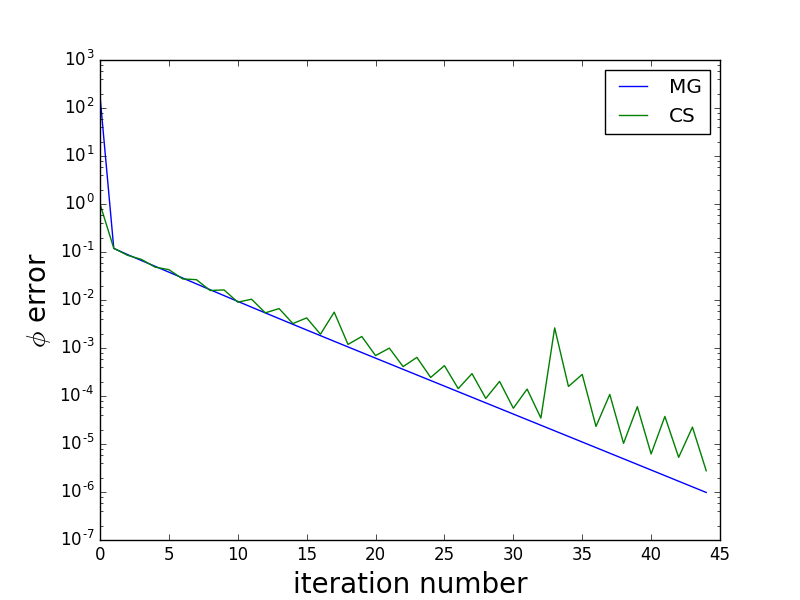
\includegraphics[width=.49\textwidth]{./graphics/phi_error_2.png}
  %\caption{640 MG groups}
\end{subfigure}
\hfill
\begin{subfigure}
  \centering
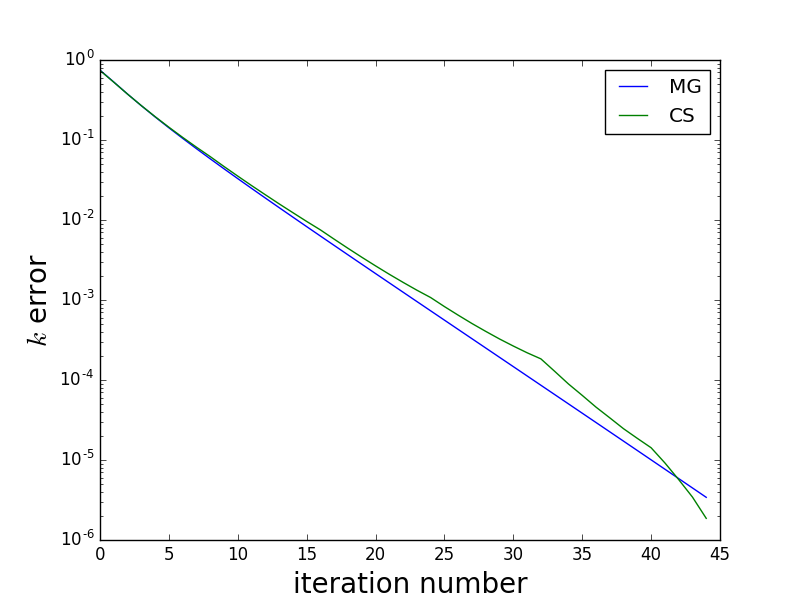
\includegraphics[width=.49\textwidth]{./graphics/k_error_2.png}
  %\caption{640 MG groups}
\end{subfigure}
\end{figure}
\end{frame}

\begin{frame}
  \frametitle{Conclusion}

\begin{itemize}
\item CS maps scattering and fission onto a coarse grid, and then maps the sourced-particle flux back onto the fine grid
\item CS converges to same solution as MG
\item CS converged almost twice as fast as MG for test problems
\end{itemize}

\end{frame}


\begin{frame}
  \frametitle{Future work}

\begin{itemize}
\item Explore possibility of maintaing particle balance in every iteration
\item Develop critera for when $S_{\ell, e \to g}$ and $F_{e \to g}$ should be recomputed
\item Try to combine CS with DSA

\end{itemize}

\end{frame}

\begin{frame}
  \frametitle{Future work: leverage properties of spherical harmonics}

\begin{figure}[ht]
  \centering
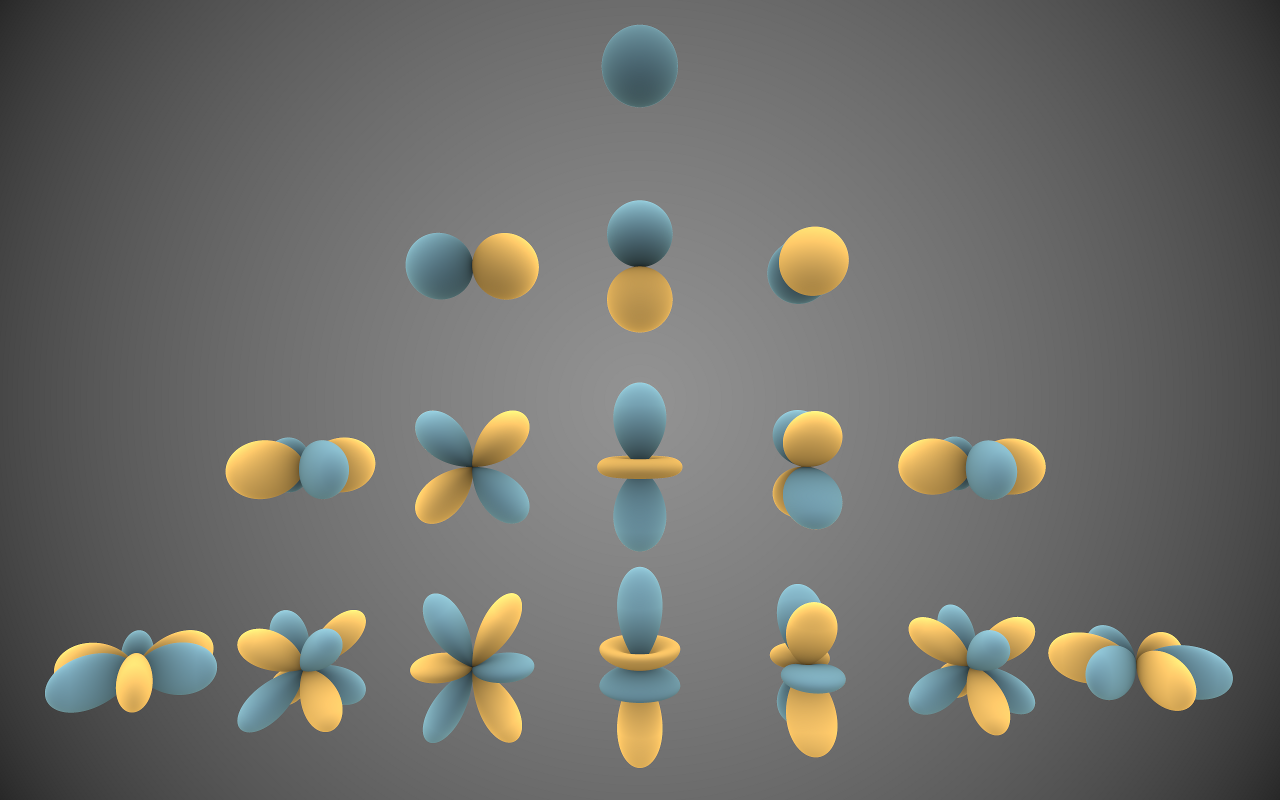
\includegraphics[width=.6\textwidth]{./graphics/Spherical_Harmonics.png}
\end{figure}

\begin{equation*}
\int_{4\pi} d\Omega \, \frac{2\ell + 1}{4\pi} Y_\ell^m(\hat{\Omega}) Y_{\ell'}^{m'}(\hat{\Omega}) =  \delta_{\ell \ell'} \delta_{m m'} 
\end{equation*}

%\begin{equation*}
%\int_{4\pi} d\Omega \, \frac{2\ell + 1}{4\pi} Y_\ell^m(\hat{\Omega}) Y_0^0(\hat{\Omega}) = \delta_{\ell 0} \delta_{m 0} 
%\end{equation*}

\begin{equation*}
\int_{4\pi} d\Omega \, \sum_{\ell = 0}^L \sum_{m=-\ell}^{\ell} \frac{2\ell + 1}{4\pi}  Y_\ell^m(\hat{\Omega}) \textcolor{blue}{Y_0^0(\hat{\Omega})} = 1
\end{equation*}

\end{frame}

\begin{frame}
  \frametitle{Future work: particle balance might be maintained in every iteration if CS is only used for higher moments}

\begin{equation*}
\int_{4\pi} d\Omega \, Y_0^0(\hat{\Omega}) \sum_{\ell = 0}^L \sum_{m = -\ell}^{\ell} \frac{2\ell + 1}{4\pi} Y_\ell^m(\hat{\Omega}) \sum_{g'}^G \Sigma_{s,\ell,g' \to g} \phi_{\ell,g'}^m = \Sigma_{s,0,g' \to g} \phi_{0,g'}
\end{equation*}

\begin{multline*}
\int_{4\pi} d\Omega \, Y_0^0(\hat{\Omega}) \Big\{ \frac{1}{4\pi} Y_0^0(\hat{\Omega}) \sum_{g'}^G \Sigma_{s,0,g' \to g} \phi_{0,g'} \: + \\ \sum_{\ell = 1}^L \sum_{m = -\ell}^{\ell} \frac{2\ell + 1}{4\pi} Y_\ell^m(\hat{\Omega}) S_{e \to g} \sum_{e'}^E \Sigma_{s,\ell,e' \to e} \phi_{\ell,e'}^m \Big\} = \Sigma_{s,0,g' \to g} \phi_{0,g'}
\end{multline*}

\end{frame}





\begin{frame}[noframenumbering]
\frametitle{Thank you}
Questions?
\end{frame}







\end{document}
